\section{Results}
\subsection{\protect\Acl{SD} classification}

The performance of the various control features is shown in
Table~\ref{tab:sd}, as well as the performance on the newly proposed \ac{SOB}
covariance features. For \acf{SD} classification, the \ac{LDA} classification of
\ac{CSP} log-variance features had the highest mean accuracy. However, there was
no significant difference between the performance of this \ac{CSP} pipeline and
direct covariance classification (whcov \ac{SVM}), and the latter had a higher
median performance (72.7\% accuracy). This demonstrates the feasibility of
direct covariance classification.
%
The \ac{logBP} features performed much worse than the spatially filtered
alternatives.
%
The \ac{SOB} features worked almost as well as the \ac{CSP} features when low
$\alpha$-values were used; with faster adaption rates the \ac{SOB} did not
perform as well with \ac{SD} application.

\begin{table}
  \caption{The \protect\acl{SD} accuracy of the different pipelines on the
  last 22 trials of each session for the 51 test subjects.}
  \center \label{tab:sd}
  \begin{tabular}{l c r@{ }l c}
\toprule
Pipeline & Half life & Mean & (std.) & Median\\
\midrule
logBP SVM && 62.2 &(11.5) & 63.6\\
CSP logvar LDA  && \textbf{69.5} &(14.6) & 68.2\\
CSP var SVM && 68.6 &(15.0) & 68.2\\
whcov SVM && 68.9 &(15.2) & \textbf{72.7}\\
SOB cov SVM (best) & 13.8 trials & 67.1 &(13.3) & 68.2\\
SOB cov SVM (worst)& 1 trial & 64.8 &(13.1) & 63.6\\
\bottomrule
\end{tabular}

\end{table}

\begin{table}
  \caption{The \protect\acl{SI} accuracy of the different pipelines on the last
  22 trials of each session for the 51 test subjects.}
  \center \label{tab:si}
  \begin{tabular}{l c r@{ }l c}
\toprule
Pipeline & Half life & Mean & (std.) & Median\\
\midrule
logBP SVM && 58.1 & (11.1) & 54.5\\
CSP logvar LDA && 59.3 & (11.8) & 54.5\\
CSP var SVM && 56.4 & (9.7) & 54.5\\
whcov SVM && 59.1 & (10.8) & 54.5\\
%SOB cov SVM & 500 & 65.9 & (13.3) & 68.2\\
%SOB cov SVM & 707 & 66.9 & (13.4) & 68.2\\
%SOB cov SVM & 793 & 67.2 & (12.7) & 63.6\\
SOB cov SVM (best) & 4.0 trials & \textbf{67.3} & (13.4) & \textbf{68.2}\\
%SOB cov SVM & 870 & 67.0 & (13.5) & 68.2\\
%SOB cov SVM & 890 & 66.9 & (13.2) & 68.2\\
%SOB cov SVM & 905 & 67.1 & (13.3) & 68.2\\
%SOB cov SVM & 917 & 66.7 & (13.0) & 63.6\\
%SOB cov SVM & 925 & 66.8 & (12.6) & 63.6\\
%SOB cov SVM & 933 & 66.7 & (12.5) & 63.6\\
%SOB cov SVM & 938 & 66.8 & (12.5) & 63.6\\
%SOB cov SVM & 943 & 66.3 & (12.8) & 63.6\\
%SOB cov SVM & 948 & 66.0 & (12.7) & 63.6\\
%SOB cov SVM & 951 & 65.3 & (13.1) & 63.6\\
%SOB cov SVM & 954 & 65.3 & (13.2) & 63.6\\
%SOB cov SVM & 957 & 65.4 & (13.0) & 63.6\\
%SOB cov SVM & 960 & 65.1 & (13.3) & 63.6\\
%SOB cov SVM & 962 & 65.1 & (13.0) & 63.6\\
SOB cov SVM (worst) & 18.9 trials & 64.9 & (13.0) & 63.6\\
\bottomrule
\end{tabular}

\end{table}

\begin{figure}
  \center 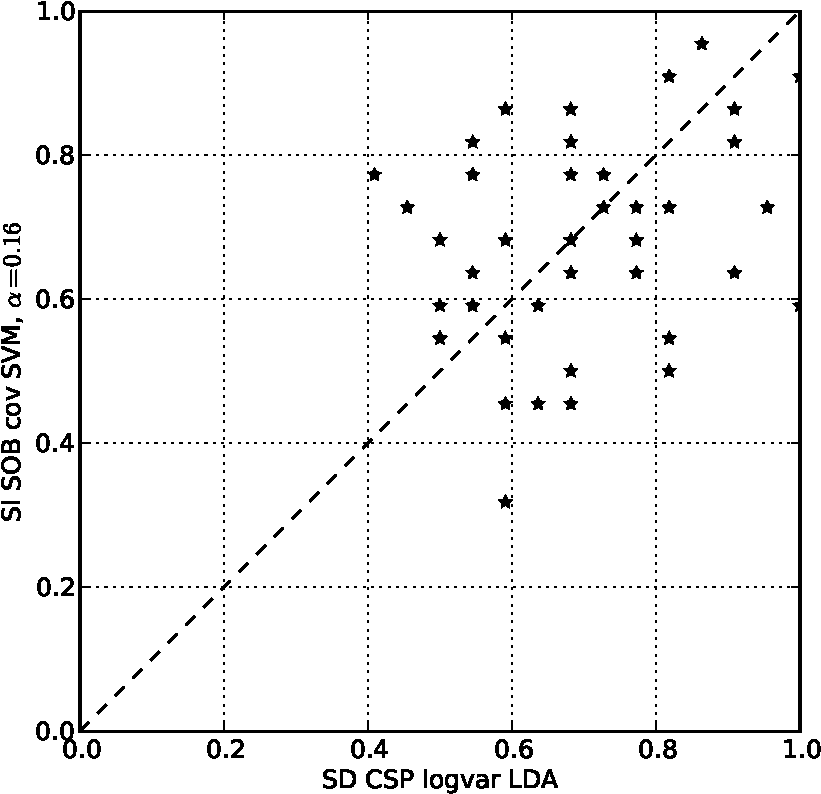
\includegraphics[width=2.3in]{sob_vs_csp.pdf} 
  \caption{The accuracy of a \protect\acl{SD} \protect\ac{CSP} pipeline versus
  the performance of a \protect\acl{SI} \protect\ac{SOB} pipeline. There is no
  significant difference between the classifiers, despite the fact that the
  \protect\ac{SOB} pipeline was not trained on the subject.}
  \label{fig:csp_vs_sob}
\end{figure}


\subsection{\protect\Acl{SI} classification}
\begin{sloppypar}
The performance of the various control methods severely degraded due to
inter-subject variability (Table~\ref{tab:si}) when these classifiers were
applied in a \acf{SI} fashion.
%
The \ac{CSP} based classifiers, which did outperform the naive \ac{logBP}
classifier with \acl{SD} training, now performed at the same level as \ac{logBP}
classifier with \ac{SI} application --- the advantage that spatial filtering
provided in the \ac{SD} training disappeared with \ac{SI} application.
%
The performance of the \ac{SOB} based predictions however, was not affected at
all. The accuracy of the best \acl{SI} \ac{SOB}-based predictions was not even
significantly different from the best \acl{SD} (\ac{CSP} log-variance \ac{LDA}
based) predictions (p=0.16 with a Wilcoxon signed-rank test on 51 paired
observations, see Fig.~\ref{fig:csp_vs_sob}).
\end{sloppypar}
 
The best \ac{SI} performance was obtained with a volatile baseline with a half
life of 4 trials, while with \ac{SD} application the best results were obtained
with long half lives (low $\alpha$'s). Note that even the worst performing
\ac{SOB} classifier outperformed all of the control classifiers.
%
Fig.~\ref{fig:csob_acc} displays the fraction of correctly classified trials as
a function of the amount of smoothing of the pre-trial baseline covariance. The
best performance was obtained with a baseline half-life between 2--11 trials.

\begin{figure}
  \center 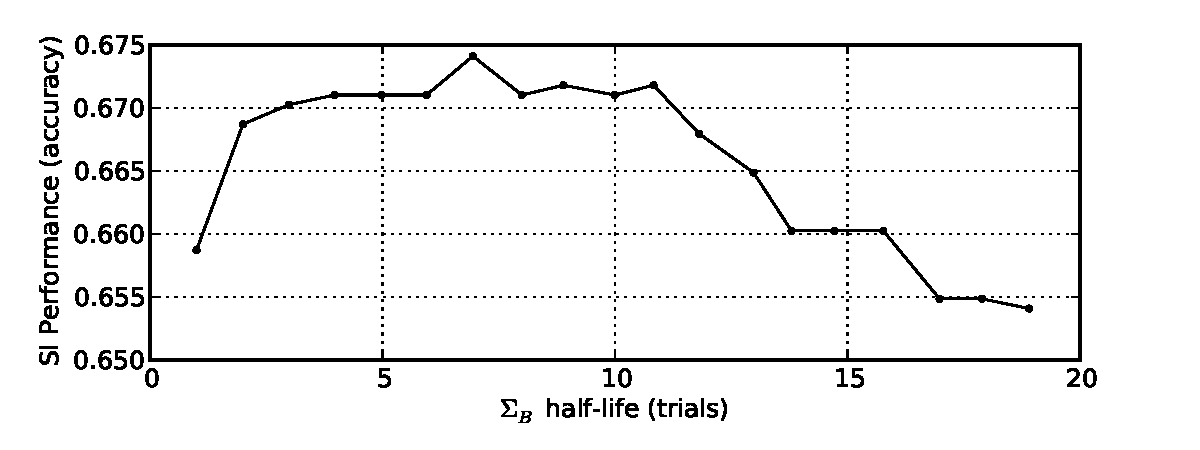
\includegraphics[width=\textwidth]{si_hl_acc.pdf} 
  \caption{The mean \protect\ac{SI} accuracy of the \protect\ac{SOB} as a
  function of the half-life of the baseline estimate $\Sigma_{B(i)}$ of the
  predictions on the last 22 trials of all the 59 test subjects. 
  }
  \label{fig:csob_acc}
\end{figure}

\begin{figure}
  \center 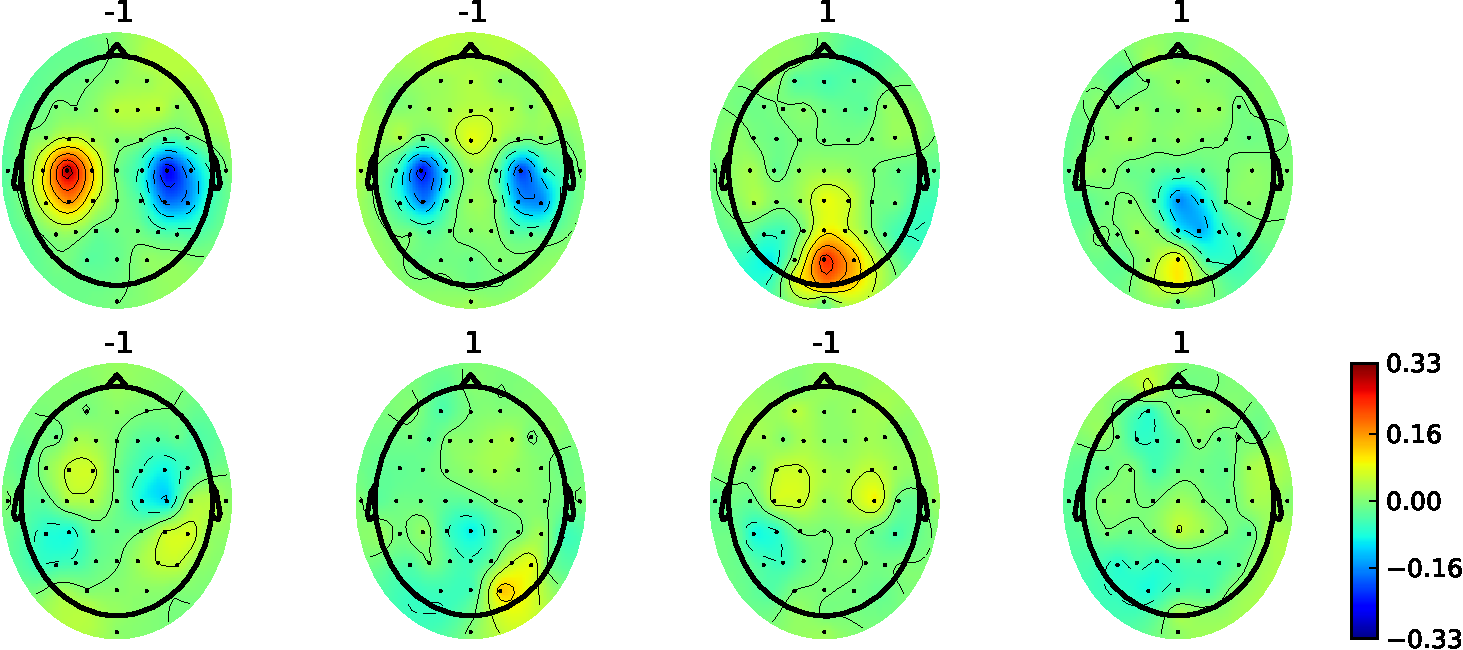
\includegraphics[width=4in]{ud_filters_scaled.pdf} 
  \caption{The most influential spatial filters $W_{i,\cdot}$ for the best
  \protect\ac{SI} \protect\ac{SOB} classifier scaled by the magnitude of their
  weight $w_i$. The number above the plot is the weight $w_i$ (i.e. a positive
  sign indicates filters with a response that corresponds to imagery of foot
  movement, a negative sign indicates imagined hand movement). Most of the
  contribution seems to originate from the motor areas, the central parietal
  regions and the visual cortex.}
  \label{fig:ud_patt}
\end{figure}

The most contributing spatial filters that were learned implicitly by the
\ac{SI} \ac{SOB} covariance classifier are shown in Fig.~\ref{fig:ud_patt}.
These filters can be easily extracted with an eigenvalue decomposition of the
covariance matrix, see \eqref{eq:filter_fac}. The most relevant features
originated from the motor cortex region, but also occipital and central
parietal features contributed to the classifiers predictions. There was no
apparent contribution of muscle or eye movement artifacts to the
classification.
